\chapter{Theoretische Grundlagen}\label{sec:basics}

In diesem Kapitel werden die für den Forschungshintergrund und die Entwicklung des Prototyps wichtigen theoretischen Grundlagen beschrieben.
Zunächst werden verschiedene Theorien zu Kommunikationsmodellen und kooperativer Kommunikation vorgestellt, die dem Modell dieser Anwendung zugrunde liegen.
Im Anschluss daran werden die in der Ludologie beschriebenen Akteurstypen vorgestellt, die sich in den Teilnehmenden dieser Masterarbeitsstudie widerspiegeln.
Allgemein ist bekannt, dass Video- und Computerspiele drei verschiedene Modi haben können: Singleplayer, Multiplayer und Mischformen. Da im Rahmen dieser Studie ein Multiplayer-Spiel konzipiert und umgesetzt wurde, werden im weiteren Verlauf verschiedene Kategorien von Multiplayer-Spielen vorgestellt. Außerdem werden die damit einhergehenden Netzwerkinfrastrukturen dargestellt, die für die aktuelle sowie eine potenzielle zukünftige Entwicklung relevant sind. Zum Schluss erfolgt ein Einblick in die \ac{AR}.

\section{Kommunikationsforschung}
Kommunikation bezeichnet den Prozess des Sendens und Empfangens von Botschaften, den Austausch von Informationen sowie die Interaktion mit anderen. Sei es im direkten persönlichen Kontakt oder über eine Vielzahl etablierter und neuer Technologien (vgl. \cite[S. 18]{krcmar_communication_2016}).
Bentele und Beck präzisieren diese Definition durch Hinzunahme, dass die wechselseitige Bedeutungsübermittlung zumeist durch sprachliche Symbole oder auch nonverbal erfolgen kann (z. B. über Blicke oder Gesten) (vgl. \cite[S. 20]{bentele_information_1994}).

\begin{quote}
\textit{\enquote{Kommunikation wird somit als soziale Interaktion zwischen zwei oder mehreren Menschen verstanden, die dem Austausch von Informationen, Gedanken, Erfahrungen etc. innerhalb einer aktuellen Situation dient.}} \cite[S. 19]{becker_praxishandbuch_2018}
\end{quote}

Sobald Menschen miteinander kommunizieren, geschieht dies i. d. R. auf mehrere Ebenen gleichzeitig. Bei den Ebenen der Kommunikation wird zwischen verbaler, paraverbaler und nonverbaler Kommunikation unterschieden. Verbale Informationen können gelesen ebenfalls einen Sinn ergeben: Nonverbale Informationen durch Mimik, Gestik und die Körpersprache können nur dann verstanden werden, wenn der Gegenüber sie sieht. Paraverbale Informationen werden durch die Betonung, Stimmlage, Pausenlängen etc. übermittelt. Sie können nur durch das Hören gedeutet werden (vgl. \cite[S. 33]{ebert_formen_2018}).

Kommunikation ist durch gegenseitige Abhängigkeiten geprägt: Während der Sender das Geschehen aktiv beeinflusst, nimmt der Empfänger Informationen auf und interpretiert sie. Dabei ist nicht jede Kommunikation bewusst beabsichtigt. Die Abgrenzung von Kommunikation und Interaktion ist schwierig, da Kommunikation meist als Teil von Interaktion verstanden wird. Kommunikatives Verhalten wird sowohl durch bewusste Erfahrungen und Lernprozesse als auch durch unbewusste Verhaltensmuster geprägt (vgl. \cite[S. 20]{becker_praxishandbuch_2018}.

Damit beschrieben werden kann, welche Prozesse innerhalb der Kommunikation geschehen, wie die Kommunikation erlebt und verstanden wird, wurden im Laufe der Zeit viele Theorien und Modelle entwickelt, die sich dieser anmahnen (vgl. \cite[S. 311]{schwarz_grundlagen_2019}).

Kommunikationsmodelle berücksichtigen stärker den sozialen Kontext. Sie sind keine exakten Abbilder der kommunikativen Realität, sondern Vereinfachungen realer Erscheinungsformen und Prozesse und Kommunikation (vgl. \cite[S. 56]{maletzke_kommunikationswissenschaft_1998}.

\subsection{Kommunikationsmodell nach Shannon / Weaver}

\begin{figure}[ht]
\centering
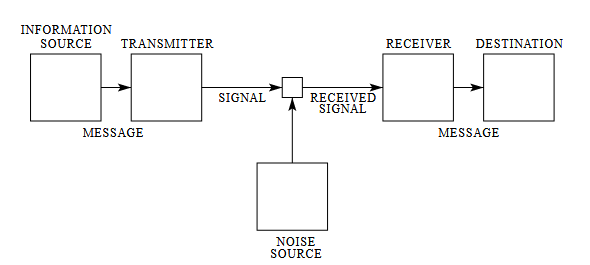
\includegraphics[width=1\linewidth]{content/pictures/shannon-weaver.PNG}
\caption{Kommunikationsmodell von Shannon / Weaver (Quelle: \cite[S. 2]{shannon_mathematical_1948})}
\label{fig:shannon-weaver-modell}
\end{figure}

Abbildung \ref{fig:shannon-weaver-modell} zeigt das wohl bekannteste Klassifikationsmodell von Shannon / Weaver. Es beschreibt jedoch keine soziale Kommunikation, sondern einen technischen Signaltransfer zwischen Sender und Empfänger. Es zeigt eine physikalische Informationsübertragung, wie z. B. ein Telefongespräch (vgl. \cite[S. 92]{scheufele_kommunikationstheorien_2004}). 

Eine Informationsquelle will eine Nachricht an ein Ziel senden. Dabei wird die Nachricht durch einen Transmitter in ein analoges/ digitales Signal umgewandelt und an ein Empfängergerät übermittelt. Innerhalb des gesendeten Signals können Störgeräusche einwirken, die ebenfalls mit übermittelt werden. Über das Empfangsgerät kann der Empfänger nun die Nachricht mitsamt Störsignal bspw. abhören.

\subsection{Kommunikationsmodell nach Osgood / Schramm}

\begin{figure}[ht]
\centering
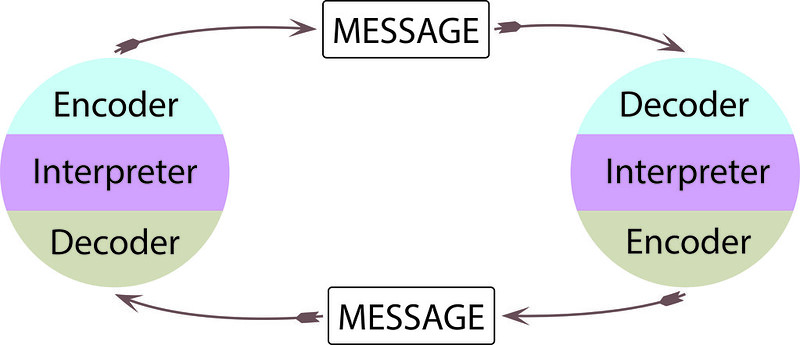
\includegraphics[width=1\linewidth]{content/pictures/osgood-schramm.jpg}
\caption{Kommunikationsmodell von Osgood / Schramm (Quelle: \cite{wrench_24_2021})}
\label{fig:osgood-schramm-modell}
\end{figure}

Das in Abbildung \ref{fig:osgood-schramm-modell} gezeigte Modell unterscheidet sich grundlegend von früheren, linearen Modellen, wie dem von Shannon / Weaver. Es zeigt stattdessen die Wechselseitige und Zirkularität von Kommunikation an. Kommunikation ist nicht nur eine einmalige Übertragung von Signalen, sondern ein kontinuierlicher Austausch, in dem beide Gesprächspartner die Bedeutung einer Botschaft gemeinsam aushandeln. Eine Antwort oder Feedback ist dabei kein optionales Element, sondern ein zentrales. Es erlaubt zudem Missverständnisse zu klären, Reaktionen einzuholen und Aussagen zu präzisieren (vgl. \cite{noauthor_osgood_2024}). 

Besonders an dem Modell ist, dass persönliche Erfahrungen der Kommunikationsteilnehmer in Form von individuellen Erfahrungen, kulturelle Prägungen, Bildung und Erwartungen in den Gesprächszyklus einfließen kann. Anhand dieser Erfahrungen erfolgt ein Codierungs / Decodierungsprozess in sprachliche und nicht-sprachliche Zeichen, welche der Empfänger interpretiert (vgl. \cite{noauthor_osgood_2024}). 

\subsection{Kommunikationsmodell nach Badura}
Als Erweiterung des Modells von Osgood und Chramm kann das Modell von Badura gesehen werden (vgl. Abbildung \ref{fig:badura-modell}).

\begin{figure}[ht]
\centering
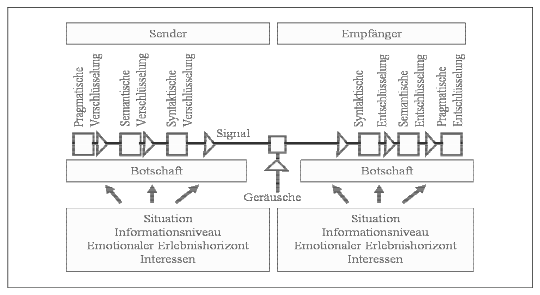
\includegraphics[width=1\linewidth]{content/pictures/badura.PNG}
\caption{Kommunikationsmodell von Badura (Quelle: \cite{badura_kommunikation_1992}, \cite[S. 93]{scheufele_kommunikation_2007})}
\label{fig:badura-modell}
\end{figure}

Das Kommunikationsmodell unterscheidet zwischen semantischen, syntaktischen und pragmatischen Aspekten der Sprache bzw. kommunikativer Botschaften. Der Rahmen in der die Kommunikation stattfindet, umfasst in diesem Modell vier Aspekte der Kommunikationssituation und zwar: dem Informationsniveau der Teilnehmer, dem emotionalem Erlebnishorizont der Teilnehmer in den jeweiligen Situationen und deren Interessen und Zielen (vgl. \cite[S. 93]{scheufele_kommunikation_2007}).

\subsection{Das Kommunikationsquadrat nach Schultz von Thun}
Während die Modelle von Shannon / Weaver oder Osgood / Schramm den Ablauf und die Zirkularität von Kommunikation erklären, geht das Kommunikationsquadrat direkt auf die inhaltliche Vielschichtigkeit jeder Botschaft ein. Sobald Menschen miteinander kommunizieren, übermitteln sie nicht nur Inhalte, sondern auch Hinweise zur Beziehung, zur Selbstdarstellung und zum kommunikativen Zweck.

\begin{figure}[ht]
\centering
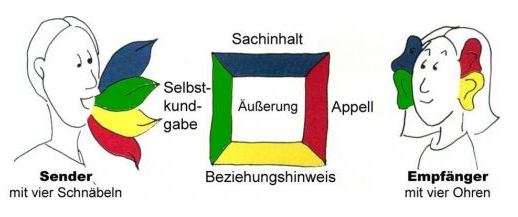
\includegraphics[width=1\linewidth]{content/pictures/Kommunikationsquadrat.PNG}
\caption{4 - Ohren Modell von Schulz von Thun (Quelle: \cite{noauthor_kommunikationsquadrat_nodate})}
\label{fig:four-ears}
\end{figure}

Das in Abbildung \ref{fig:four-ears} gezeigte Modell, auch \say{Nachrichtenquadrat} oder \say{Kommunikationsquadrat}, genannt, zeigt die vier Botschaften, die eine Nachricht gleichzeitig enthält. Diese sind die Sachinformation, bei der darüber informiert wird, um was es in der Nachricht geht. Die Selbstkundgabe, bei der der Sender Informationen über sich selbst freigibt. Dem Beziehungshinweise, in welchem Verhältnis der Sender zum Empfänger steht und den Appell, durch welchen das Ziel der Botschaft offenbart wird (vgl. \cite{noauthor_kommunikationsquadrat_nodate}).

Die gewählten Äußerungen entstammen dabei aus den \say{vier Schnäbeln} des Senders, die auf die \say{vier Ohren} des Empfängers treffen (vgl. \cite{noauthor_kommunikationsquadrat_nodate}). Schulz von Thun geht dabei davon aus, dass jede Nachricht mit vier Ohren empfangen werden (vgl \cite[S. 23]{becker_praxishandbuch_2018}). 

Dieses Modell ist im Kern ein Ausdrucksmodell der Kommunikation. Einerseits soll es dabei dabei helfen, Ursachen für mögliche Missverständnisse zu verstehen und andererseits übersieht es den Charakter der Gemeinschaftshandlung als auch den Steuerungscharakter des Sprechens (vgl \cite[S. 23]{becker_praxishandbuch_2018}). Es berücksichtigt somit nicht das Nachfragen beim Sender. Stattdessen suggeriert es, dass jede Äußerung einen einzigen wahren Bedeutungskern hätte (vgl \cite[S. 23]{becker_praxishandbuch_2018}). 

\subsection{Konversationsmaximen von Grice}
Grice erweitert die o. g. Theorien dadurch, dass nicht nur über das Gesagte die Kommunikation funktioniert, sondern auch durch das Implizierte (vgl. \cite[S. 43f]{grice1975logic}). Aus den Bedingungen unter welchen Konversationen stattfinden. In  der Regel bestehen sie nicht aus zufälligen und unzusammenhängenden Äußerungen, sondern man kann das Kooperationsprinzip ableiten. Es handelt dabei davon, dass der Gesprächsbeitrag so gestaltet werden soll, wie es der Zweck oder die Richtung des Gesprächs in dem jeweiligen Stadium verlangt (vgl. \cite[S. 45]{grice1975logic}).
Aus dieser Annahme können vier Kategorien unterschieden werden. Die Quantität (Menge der Informationen) beinhaltet, dass der (gesprochene) Beitrag so informativ wie erforderlich, jedoch nicht informativer als nötig gestaltet werden soll. Die Qualität (Wahrheit) beinhaltet die Aufrichtigkeit der Nachricht. Es darf nichts gesagt werden, was der Sprecher für falsch hält und wofür keine ausreichende Belege vorhanden sind. Unter dieser Relation wird die Relevanz der Nachricht definiert. Und zuletzt: die Modalität (Art und Weise) des Gesagten. Darunter fallen die Vermeidung von Unklar- und Mehrdeutigkeiten, sowie das Vermeiden von Ausschweifungen und die Forderung nach Ordnung (vgl. \cite[S. 45f]{grice1975logic}).

Sobald gegen eine der Maximen verstoßen wird, kann der andere Interaktionsteilnehmer davon ausgehen, dass es dafür einen Grund gibt. Hier entsteht nun die implizierte Bedeutung. Die Maximen können den Kommunikationsteilnehmern eine Interpretationshilfe geben (vgl. \cite[S. 49f]{grice1975logic}).

\subsection{Axiome der Kommunikationen nach Watzlawik et. al}
In Ergänzung zu den zuvor genannten Modellen betrachten Watzlawik, Beavin und Jackson die Grundlagen zwischenmenschlicher Kommunikation aus der systematisch konstruktivistischen Perspektive. Im Zentrum steht die Kommunikation als wechselseitiges Verhalten innerhalb sozialer Kontexte (vgl. \cite{Watzlawick2016-km}). 

Dabei wurden fünf Grundsätze (Axiome) definiert, die die menschliche Kommunikation erklären (vgl. \cite{Watzlawick2016-km}):
\begin{itemize}
    \item \say{Man kann nicht nicht kommunizieren}, dies wird über das Verhalten begründet, welches immer gegeben ist (vgl. \cite[S. 53]{Watzlawick2016-km}).
    \item \say{Jede Kommunikation hat einen Inhalts- und einen Beziehungsaspekt, derart, dass letzterer den ersteren bestimmt und daher eine Metakommunikation ist.} \cite[S. 64]{Watzlawick2016-km}
    \item \say{Die Natur einer Beziehung ist durch die Interpunktion der Kommunikationsabläufe seitens der Partner bedingt.} Die Kommunikation verläuft zirkular. (vgl. \cite[S. 69]{Watzlawick2016-km})
    \item Menschliche Kommunikation nutzt sowohl digitale als analoge Ausdrucksformen. Digitale Kommunikation ist logisch strukturiert, aber in Beziehungssituationen bedeutungsarm. Analoge Kommunikation hingegen transportiert Beziehungsinhalte wirkungsvoll, ist jedoch weniger eindeutig in der Bedeutung (vgl. \cite[S. 77]{Watzlawick2016-km}).
    \item \say{Zwischenmenschliche Kommunikationsabläufe sind entweder symmetrisch oder komplementär, je nachdem, ob die Beziehung zwischen den Partnern auf Gleichheit oder Ungleichheit beruht} \cite[S. 80]{Watzlawick2016-km}
\end{itemize}

\subsection{Gelingende Kommunikation nach Carl Rogers}
Die o. g. Modelle bezogen sich auf den strukturellen Aufbau und Regeln kommunikativen Handelns, sowie dem Aufbau der übermittelten Nachrichten. Carl Rogers ging einen Schritt weiter und beschäftigte sich damit, wie die Kommunikation der Teilnehmer gelingen kann (empathische Kommunikation). 

Er stellte dabei die drei wichtigen Prinzipien der Echtheit (Kongruenz), Empathie und Wertschätzung (Bedingungslose Akzeptanz) fest. Die Echtzeit umschreibt die Offenheit der Gesprächsteilnehmer, sowie die Vermeidung von Künstlichkeit im Verhalten dem anderen gegenüber. Dadurch soll ein Gefühl von Sicherheit entstehen. Die Empathie beschreibt das Hineinversetzten in die Lage des anderen. Dadurch soll versucht werden, die Gefühle und Gedanken aus den Perspektiven der Gesprächsteilnehmer zu verstehen. Dieses Verständnis fördert eine tiefere emotionale Verbindung. Die Wertschätzung umfasst, wie es das Wort bereits aussagt, das Wertschätzen der anderen Person, unabhängig seines Verhaltens oder Meinung. Aus der Wehrschätzung heraus sollen sich die Gesprächsteilnehmer sicher und geschützt fühlen (vgl. \cite{jesse_carl_2025}).
% Zunächst definierte er das Menschenbild über die Kernelemente der Selbstverwirklichung, Bedürfnisse, Individualitäten, Erfahrungen und Positivität (vgl. \cite{warkentin_carl_2024}). 
 
\section{Spielertypen}
Die Kommunikationswissenschaft umfasst zwar den Schwerpunkt dieser Arbeit, jedoch wurden auch ludologische Aspekte berücksichtigt. Dabei handelt es sich um die wissenschaftliche Auseinandersetzung mit dem Spielen selbst (vgl. \cite{ludologie_spielforschung_nodate}). 

Im Hinblick auf die Konzeption und Entwicklung eines Spiels ist es wichtig, die Eigenschaften des Spielsystems so zu gestalten, dass sie Begeisterung und Engagement bei der gewünschten Zielgruppe hervorrufen. Aus diesem Grund muss zunächst die Zielgruppe in verschiedene Typen eingeteilt werden. Die Ludologie unterscheidet hierfür verschiedene Spielertypen. Zwar ist nicht jeder Mensch ein \say{Spielertyp}, dennoch kann er grundsätzlich durch unterschiedliche Spielelemente angesprochen werden (vgl. \cite{ludologie_spielertypen_nodate}).

\subsection{Nach Bartle}
1996 beschäftigte sich Richard Bartle mit der Frage, welche Spielertypen in der Ludologie unterschieden werden können. Dabei ging es zunächst um Klassifizierungen von Ansätzen, die beim Spielen von sogenannten \ac{MUD}s existieren (vgl. \cite{bartle_hearts_1996}). Diese Klassifizierungen werden noch heute für die Einteilung in Spielertypen herangezogen.

Bartle unterscheidet bei der Einteilung der Spielertypen zwei grundlegende Interessen (vgl. Abbildung \ref{fig:bartle-muds}):

\begin{figure}[ht]
\centering
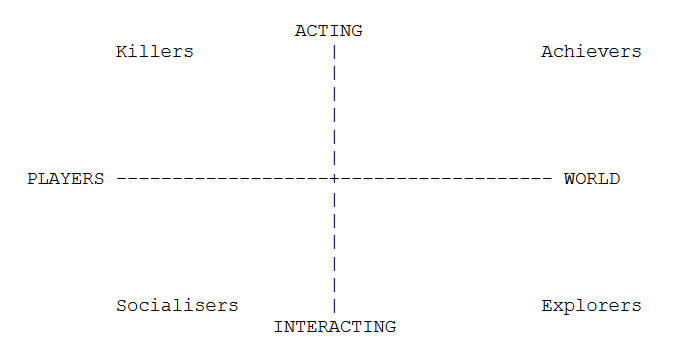
\includegraphics[width=1\linewidth]{content/pictures/basic_interests.PNG}
\caption{Interessen Graph nach Bartle (Quelle: \cite{bartle_hearts_1996})}
\label{fig:bartle-muds}
\end{figure}

Auf der X-Achse wird unterschieden, ob Spieler ihre Spielerfahrung über das Verhalten der anderen Mitspieler (Players) oder über die Spielwelt (World) definieren. Entlang der Y-Achse wird unterschieden, ob Spieler eher selbst aktiv Einfluss auf die Spielwelt nehmen möchten (Acting) oder ob sie in eine tiefere Interaktion mit ihr eingehen wollen (Interacting).

Die daraus resultierenden Typen sind:
\paragraph{Achiever}
Sie sind daran interessiert, auf die Spielwelt einzuwirken und alle ihnen gestellten Aufgaben mit Erfolg zu absolvieren. Ihr Status im Spiel ist ihnen wichtig - ebenso wie die Effizienz, mit der sie Fortschritte erzielen.

\paragraph{Explorer}
Sie wollen vom Spiel überrascht werden und intensiv mit der Spielwelt interagieren. Die virtuelle Welt löst ein Gefühl des Staunens aus, nach dem sie aktiv suchen. Sie sind stolz auf das Wissen, das sie im Spiel sammeln. Das erlangte Wissen möchten sie gerne an neue Spieler weitergeben.

\paragraph{Socialiser}
Sie wollen mit anderen Spielern interagieren, meist über Gespräche, aber auch durch ungewöhnliche oder kreative Verhaltensweisen. Andere Menschen kennenzulernen und mehr über sie zu erfahren, ist für sie wertvoller als für andere. Die Spielwelt dient dabei lediglich als Kulisse - entscheidend sind für sie die Begegnungen mit anderen Charaktere. Sie sind stolz auf Freundschaften, ihre Kontakte und ihren Einfluss.

\paragraph{Killer}
Sie sind daran interessiert, auf andere Spiele einzuwirken und mit ihnen zu interagieren - häufig ohne deren Einverständnis. Sie wollen ihre Überlegenheit gegenüber anderen Menschen demonstrieren und sind stolz auf ihren Ruf sowie ihre oft geübten Kampffähigkeiten.

(vgl. \cite{bartle_hearts_1996}).

\subsection{Erweiterte Einteilungen}
Bartle ist nicht der Einzige, der sich mit Spielertypen auseinandergesetzt hat. Seine Forschung bildet jedoch ein grundlegendes Fundament, das in der weiteren wissenschaftlichen Auseinandersetzung intensive Diskussionen innerhalb der Forschungs- und Game-Design-Community ausgelöst hat. 
\begin{quote}
    \textit{
        \enquote{Player types are not a defined concept and any categorization of players or users needs to occur within the context of a particular application or domain. Play-personas are suggested as a useful tool that can be used to put player type research into practice as part of the design process of gamified systems.}
    } 
    (\cite{dixon_player_nodate})
\end{quote}

\paragraph{Dixon} 
stellt Spieler-Personae vor, die analog zum \ac{UCD}-Prozess eingesetzt werden können. Dadurch muss im Designprozess nicht strikt zwischen Motivation, Verhalten und Vorlieben unterschieden werden, da Personae als ausführliche, erzählerische Darstellung gedacht sind (vgl. \cite{dixon_player_nodate}).

\paragraph{Bateman und Boon}
entwickelten in ihrer 2005 erschienenen Studie zur Bestimmung des ersten Modells des Demographic Game Design (DGD1) vier Spielstile, die sie durch die Einbeziehung des \ac{MBTI} ableiteten (vgl. \cite{noauthor_mbti_nodate}; \cite{bateman_21st_2005}).
% Conquerer (Eroberer), Manager, Wanderer (Wanderer) und Participant (Teilnehmer) waren dabei die vier Spielstile.
Die vier Spielstile lauteten: Conquerer (Eroberer), Manager (Manager) Wanderer (Wanderer) und Participant (Teilnehmer).

In einer zweiten Studie wurden vier hypothetische Spielstile entwickelt, die auf einer Untersuchung von \cite{berens_understanding_2000} basierten (vgl. \cite{bateman_player_2012}). Die daraus resultierenden Stile lauteten: Logistical, Tactical, Strategic und Diplomatic.

Im Kern sind diese Modelle Weiterentwicklungen bzw. Ableitungen von Bartles ursprünglicher Typologie (vgl. \cite{ludologie_spielertypen_nodate}).

\paragraph{Yee}
Nick Yee entwickelte ein empirisch fundiertes Modell zur Beschreibung von Spielmotivationen in Online-Spielen, das bis heute einen bedeutenden Einfluss auf die Ludologie hat. Anhand eines faktorenanalytischen Ansatzes untersuchte er eine Vielzahl an Daten aus Online-Umfragen und identifizierte dabei zehn spezifische Motivationsgruppen, die sich in drei übergeordnete Hauptkategorien einordnen lassen (vgl. Abbildung \ref{fig:nick_yee_motivations}):

\begin{figure}[ht]
\centering
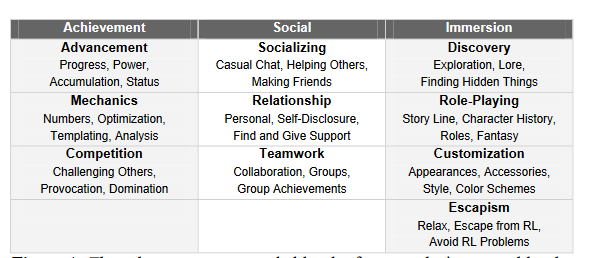
\includegraphics[width=1\linewidth]{content/pictures/nick_yee_categorizations.PNG}
\caption{Motivationsgruppen nach Nick Yee (Quelle: \cite{yee_motivations_2006})}
\label{fig:nick_yee_motivations}
\end{figure}

Die Achievement-Komponente umfasst den Fortschritt im Spiel, sowie das damit einhergehende Verlangen Macht zu erlangen, schnell voranzukommen und Symbole für Reichtum oder Status zu erwerben. Zudem besteht ein Interesse daran, die Spielmechanik zu analysieren, die Regeln und Systeme zu verstehen um die Leistung der Spielfigur zu optimieren. Auch ist der Wettbewerb spielt eine zentrale Rolle: Es besteht der Wunsch, sich mit anderen zu messen und gegen sie anzutreten.

Die soziale Komponente beschreibt das Bedürfnis nach Sozialisierung. Spieler haben Interesse daran, anderen zu helfen und sich mit ihnen zu unterhalten. Daraus entstehen Beziehungen, bei denen der Wunsch besteht, langfristige und bedeutungsvolle Bindungen zu anderen aufzubauen. Teamarbeit ist dabei gewünscht, um gemeinsame Ziele zu erreichen oder sich im Wettbewerb zu behaupten.

Die Immersion-Komponente beschreibt das Entdecken der Spielwelt und das damit verbundene Finden von Objekten sowie das Erlangen von Wissen, das den meisten anderen Spielern unbekannt ist. Rollenspiel-Elemente sind besonders wichtig, um den Spielfiguren Hintergrundgeschichten zu geben und gemeinsam improvisierte Erzählungen zu entwickeln. Der Spielavatar sollte zudem anpassbar sein, damit persönliche Vorlieben und der individueller Stil der Spieler zum Ausdruck kommen können. Die Spielwelt dient auch als Mittel um dem Alltag zu entfliehen und den Problemen der realen Welt zu entkommen.

\paragraph{weitere Modelle}
Im Zuge der fortschreitenden Forschungen entstanden weitere Modelle wie zum Beispiel das Gamer Motivation Model, das auf Basis der Forschung von Nick Yee entwickelt wurde (vgl. \cite{ludologie_spielertypen_nodate}):

\begin{figure}[ht]
\centering
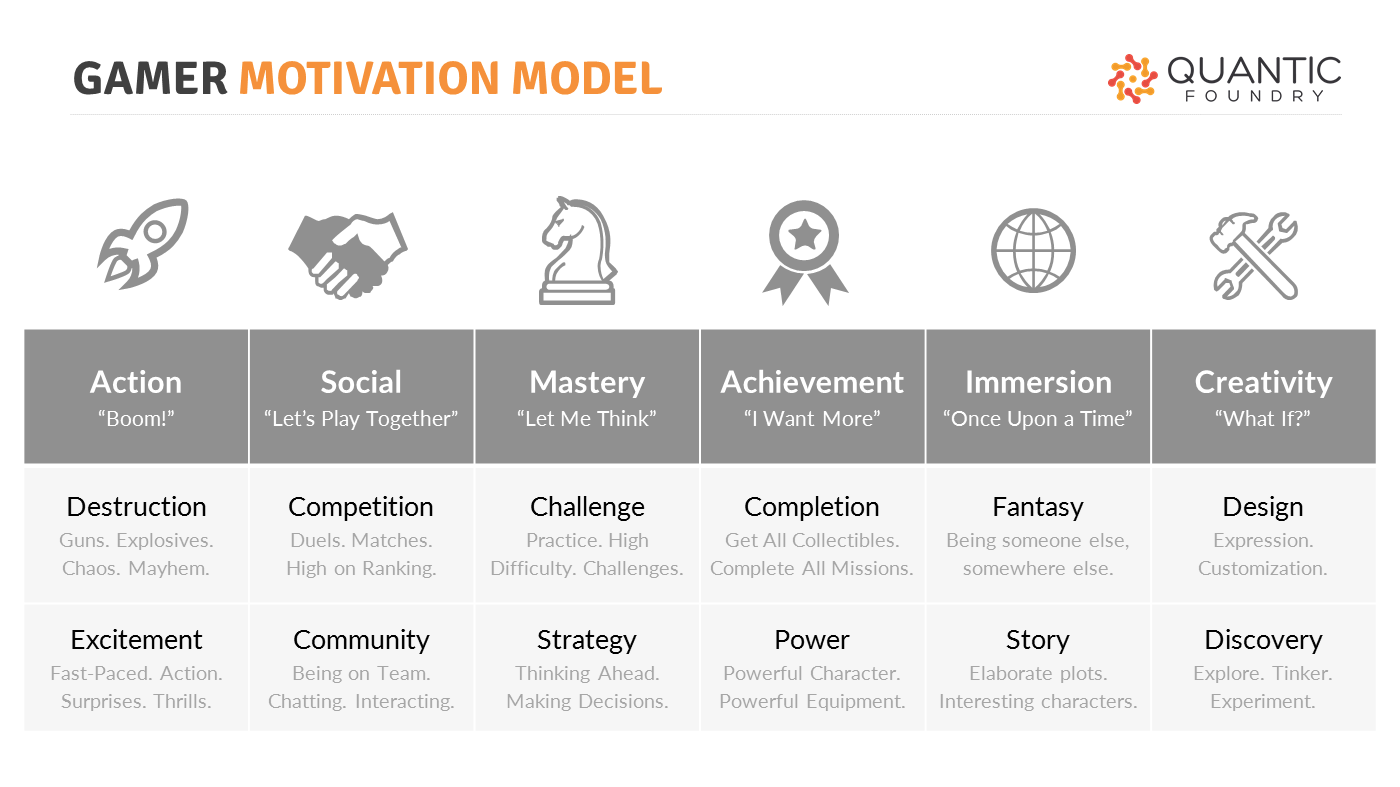
\includegraphics[width=1\linewidth]{content/pictures/gamer_motivations_model.png}
\caption{Gamer Motivation Model der QUANTIC FOUNDRY (Quelle: \cite{noauthor_quantic_nodate})}
\label{fig:gamer_motivation_model}
\end{figure}

Ein weiteres Modell, das in der Arbeit von Bateman genannt wird, ist das BRAINHEX-Model, bei dem die verschiedenen Spielertypen in hexagonaler Anordnung platziert sind (vgl. Abbildung: \ref{fig:brain-hex}):

\begin{figure}[ht]
\centering
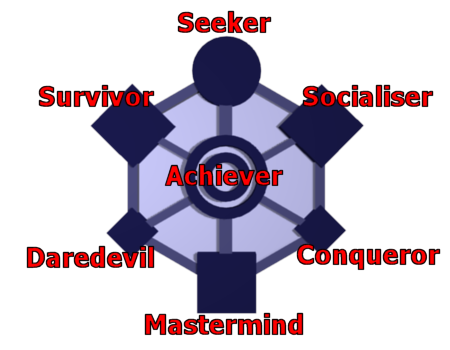
\includegraphics[width=1\linewidth]{content/pictures/brainhex-classes.png}
\caption{Brainhex-Model Darstellung von \cite{noauthor_i_nodate} nach \cite{nacke_brainhex_2013}}
\label{fig:brain-hex}
\end{figure}

\section{Multiplayer-Spiele}
Im Vergleich zu Einzelspieler-Spielen existieren bei Multiplayer-Spielen nicht nur Unterschiede im Genre, sondern auch in den Spielrollen (Symmetrie / Asymmetrie) sowie in den Spielzeitpunkten, zu denen die Spielteilnehmer an ihrem Spielfortschritt weiterarbeiten (Synchron / Asynchron). [Hier wäre eine Quelle noch gut]. Auf dem Spielemarkt existieren außerdem Multiplayer-Spiele, die unterschiedliche Medientechniken verwenden. Teilweise dienen diese Medientechniken dazu, Cross-Plattform Funktionalität zu gewährleisten (vgl. \cite{noauthor_baldurs_nodate}), oder sie sind integrale Bestandteil des Gamedesigns (vgl. \cite{noauthor_keep_nodate}).

Da im Kontext von \say{Connecting-Minds} die Spieler zeitgleich in einer Sitzung gemeinsam spielen, wird im Folgenden auf die Symmetrie und Asymmetrie von Computer- und Videospielen eingegangen.

\subsection{Symmetrische Multiplayer}
Symmetrische Spiele sind solche, bei denen alle Spieler die gleichen Spielregeln haben und das gleiche Spielziel verfolgen. Viele traditionelle Spiele wie Schach sowie Computer- und Videospiele wie \say{Mario Kart} oder \say{Minecraft} sind symmetrische Multiplayer-Spiele, bei denen für jeden Spieler das gleiche Ziel gilt (vgl. \cite[S. 12]{adams_fundamentals_2013}); (vgl. \cite{nintendo_mario_1992}); (vgl. \cite{noauthor_willkommen_2009}). 


\subsection{Asymmetrische Multiplayer}
Asymmetrische Spiele hingegen können unterschiedlichen Spielern unterschiedliche Regeln zugestehen und ggf. verfolgen die Spieler unterschiedliche Ziele (vgl. \cite[S. 12]{adams_fundamentals_2013}). Sie sind sowohl in kooperativen als auch kompetitiven Spielen weit verbreitet und werden bspw. in Form verschiedener \say{Helden} oder \say{Klassen} umgesetzt. So gibt es z.B. in \say{Overwatch} oder \say{League of Legends}  unterschiedliche \say{Support}-Charaktere, deren Aufgabe es ist das Team zu heilen (vgl. \cite{smilovitch_birdquestvr_2019}); (vgl. \cite{noauthor_league_2025}); (vgl. \cite{noauthor_overwatch_nodate}). 
Außerdem ermöglichen asymmetrische Spiele, dass Spieler mit unterschiedlichen Fähigkeiten und Fähigkeitsniveaus gemeinsam spielen können. Ein asymmetrisches Design kann zudem die Inklusivität in Spielen fördern (vgl. \cite{smilovitch_birdquestvr_2019}).

\subsection{Hybride Multiplayer}
Wie Lotz in ihrer Bachelor-Arbeit beschrieben hat, unterscheiden sich Multiplayer auch in der verwendeten Medientechnik (vgl. \cite[S. 6f]{lotz_konzeption_2021}). Sogenannte hybride Spiele wie \say{New Super Mario Bros U} (vgl. \cite{noauthor_mario_nodate-1})

\begin{figure}[ht]
\centering
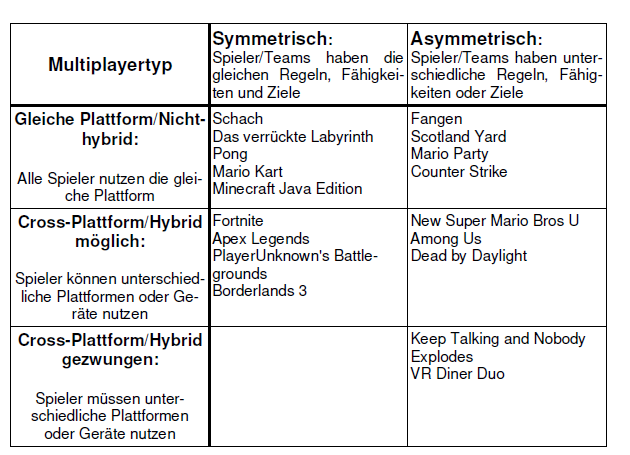
\includegraphics[width=1\linewidth]{content/pictures/lotz_hybrid_multiplayer.PNG}
\caption{Unterscheidung Multiplayertypen (Quelle: \cite[S.6]{lotz_konzeption_2021})}
\label{fig:lotz_multiplayer_types}
\end{figure}

Wie Abbildung \ref{fig:lotz_multiplayer_types} zeigt, können Multiplayer-Spiele hinsichtlich ihrer Medientechnik in drei Kategorien eingeteilt werden.
Spiele wie \say{Mario Kart} oder \say{Minecraft} können nur auf der gleiche Plattform gespielt werden. Bei Spielen wie \say{Among Us} oder \say{Fortnite} ist die Plattform, auf der gespielt wird, nicht relevant, da eine Cross-Play-Funktionalität gegeben ist. Jeder kann mit Spielern auf der Plattform spielen, die er zu zuhause hat. Die dritte Kategorie umfasst Spiele, bei denen die Spieler gezwungen werden, unterschiedliche Plattformen zu nutzen. In \say{Keep talking and nobody explodes} ist dies der Kern des Gamedesigns.

\section{Spielweisen von Multiplayer-Spielen}
Nachdem die unterschiedlichen Strukturen und technischen Formen von Multiplayer-Spielen behandelt wurden, ist es nun wichtig, die verschiedenen Spielweisen zu betrachten. Multiplayer-Spiele können dabei in drei Hauptspielformen unterteilen:
In kompetitive, kollaborative und kooperative Spielweisen (vgl. \cite[S. 25f]{zagal_collaborative_2006}).

\subsection{Kompetitiv}
Kompetitive Spiele sind solche, bei denen Spieler oder Teams gegeneinander antreten, um ein bestimmtes Ziel zu erreichen, wobei der Erfolg des einen oft den Misserfolg des anderen bedeutet. In diesen Spielen ist das Spiel selbst neutral und agiert nicht aktiv im Wettbewerb (vgl. \cite{noauthor_game_2014}), (vgl. \cite[S. 25]{zagal_collaborative_2006}).

\subsection{Kollaborativ}
Kollaborative Spiele sind solche, bei denen alle Spieler - ähnlich wie in Kooperationsspielen - gemeinsam gegen das Spiel verlieren können. Allerdings können sie nicht gemeinsam gewinnen. Diese Spiele sind im Kern meist kompetitiv, beinhalten jedoch die Möglichkeit einer kollektiven Niederlage. Die Spieler müssen zu einem gewissen Maß zusammenarbeiten, um nicht zu verlieren (vgl. \cite{noauthor_game_2014}), (vgl. \cite[S. 25]{zagal_collaborative_2006}).

\subsection{Kooperativ}
Bei Kooperationsspielen ist es möglich, dass alle Spieler gemeinsam gegen das Spiel verlieren oder gemeinsam gewinnen können. Ein Sieg wird erreicht, wenn das Spiel gemeinsam \say{besiegt} wird oder dadurch dass ein festgelegtes Ziel kollektiv oder individuell erreicht werden kann (vgl. \cite{noauthor_game_2014}), (vgl. \cite[S. 25]{zagal_collaborative_2006}).

\section{Augmented Reality}

\ac{AR} stellt eine Form virtueller Umgebungen (\ac{VE}) dar, bei der im Gegensatz zur vollständigen Immersion in rein virtuelle Welten, wie es in \ac{VR} der Fall ist, die Umgebung weiterhin sichtbar bleibt. Virtuelle Objekte werden dabei über die physische Welt gelegt und mit ihr kombiniert, sodass eine erweiterte Wahrnehmung entsteht. Es gewährleistet außerdem eine Interaktion mit den räumlich (\ac{3D}) registrierten virtuellen Inhalten in Echtzeit. Die technische Umsetzung kann dabei über monitorbasierte Schnittstellen, monokulare Systeme oder durchsichtige \ac{HMD}s erfolgen (vgl. \cite{azuma_survey_1997}).

Es gibt drei verschiedene Ansätze, wie virtuelle Objekte in die virtuelle Szene der Anwendung platziert werden können:
\begin{itemize}
    \item Marker basiertes \ac{AR}
    \item Markerloses \ac{AR}
    \item Hybride \ac{AR} Ansätze
\end{itemize}
% Der Marker-Basierte Ansatz verwendet einen bestimmten Marker um das \ac{3D}-Objekt an eine bestimmte Position zu binden. Dies kann entweder über eine Hyperlink Verknüpfung oder Visuell-Basierenden Markern geschehen. Bei der Hyperlink-Verknüpfung wird bein physisches Objekt mit einem Web-basierendem Inhalt durch graphische Tags oder Radiofrequenz-Identifikationssysteme verbunden. Die visuell-basierte Methode funktioniert durch das erkennen und verarbeiten von bestimmten Markern, wie physische Objekte in der Umgebung oder Papier-basierende Muster, durch die Kamera (vgl. \cite[S. 3f]{el_barhoumi_assessment_2022}).

% Der Markerlose Ansatz lässt sich in zwei verschiedene Typen unterteilen. Das sensorbasierte Tracking nutzt entweder das magentische Tracking-Verfahren, bei dem ein elektromagnetisches Feld und Sensoren verwendet werden um die Position und Orientierung in Echtzeit zu bestimmen. Es funktioniert unabhängig von Sichtverbindungen und ist unempfindlich gegenüber optischen Störungen. Es hat allerdings eine begrenzte Reichweite und ist störanfällig gegenüber Magnetfeldern. Das interiale Tracking verwendet.



\subsection{Abgrenzung der Begriffe}

\subsection{Technologien}

\section{Netzwerkinfrastrukturen}\label{sec:basics-network-structures}
Um ein Multiplayer-Spiel entwickeln zu können, muss zunächst geklärt werden, wie die Netzwerkinfrastruktur der Anwendung aufgebaut sein soll. Es existieren zahlreiche Ansätze, die jeweils für verschiedene Anwendungszwecke konzipiert sind.

\subsection{Distributed Authority}
Bei einer \say{Distributed Authority}-Netzwerktopologie übernimmt jeder im Netzwerk verbundene Spielclient gemeinsam jeweils die Verantwortung für das Erstellen und Verwalten von Objekten im Netzwerk. Jeder Client simuliert dabei seinen Teil der Spielwelt selbst und steuert Objekte über die er Autorität besitzt.
Damit Positionen und andere relevanten Daten an alle anderen Clients im Netzwerk weitergeleitet werden können, wird ein zentraler, leichtgewichtiger Statusdienst verwendet, der ausschließlich für die Verteilung der notwendigen Informationen zuständig ist, ohne selbst die Anwendung zu simulieren (vgl. \cite{noauthor_distributed_2025}).

\begin{figure}[ht]
\centering
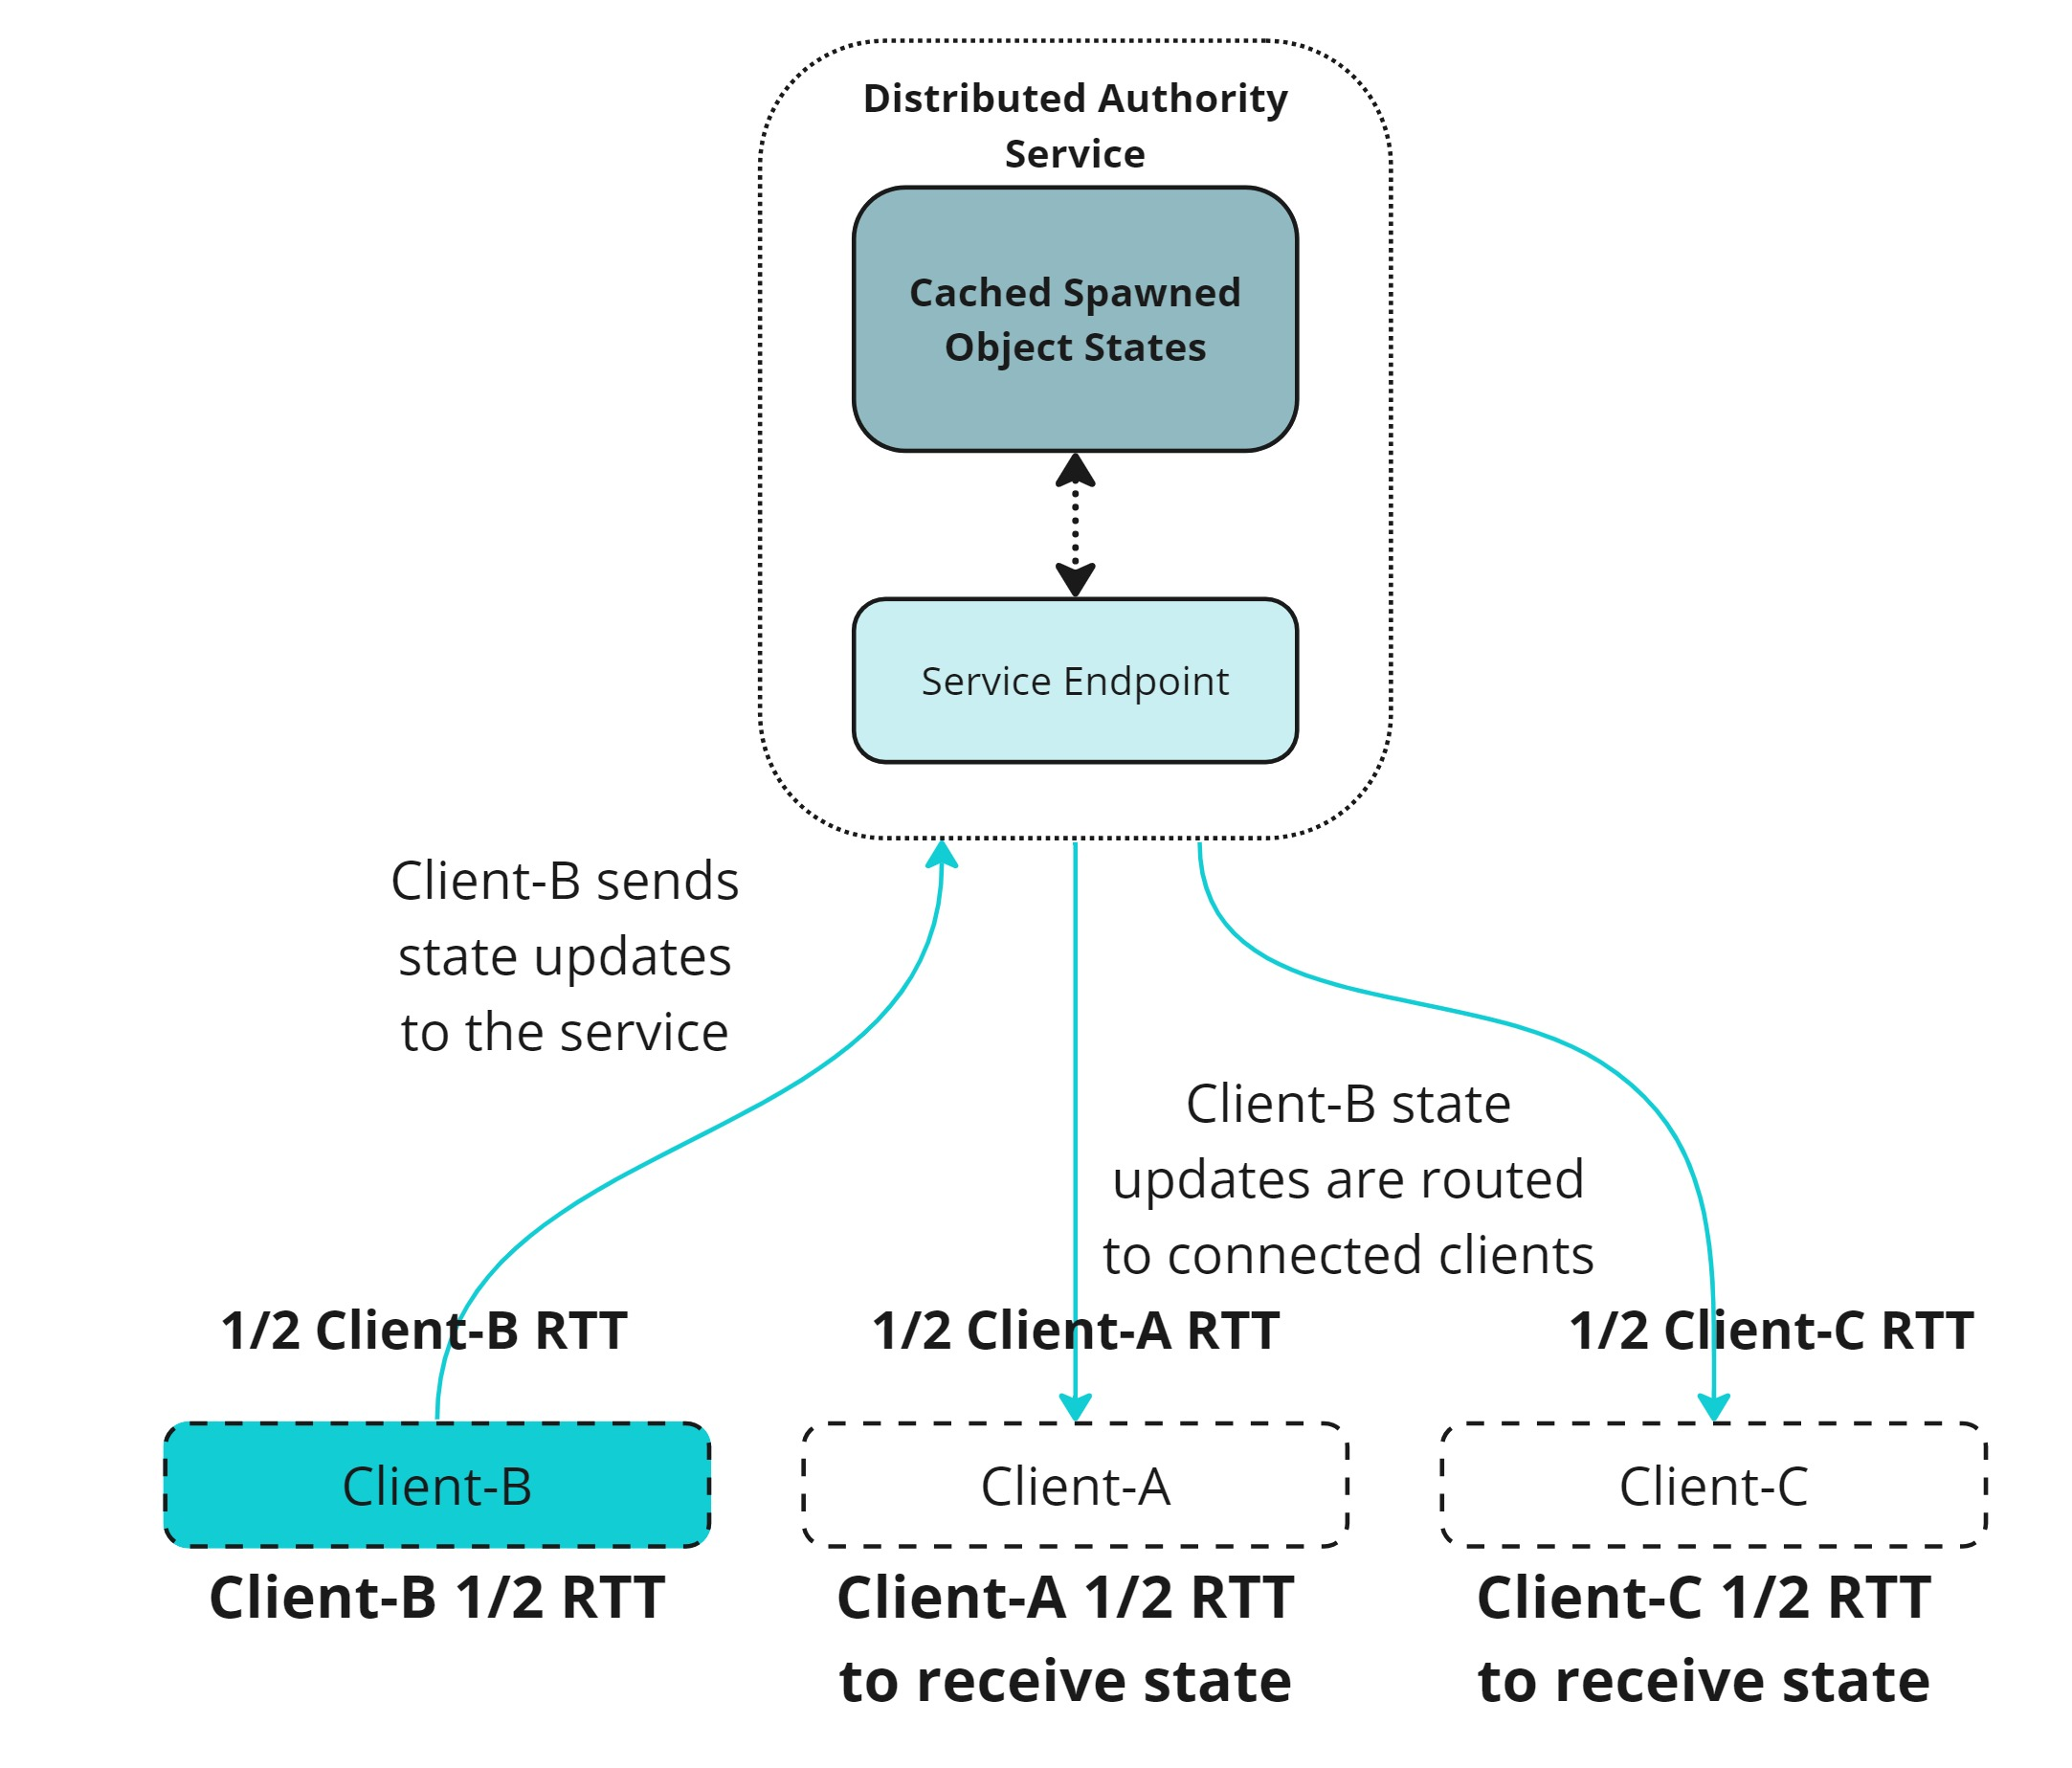
\includegraphics[width=1\linewidth]{content/pictures/distributed-authority-service.jpg}
\caption{Netzwerktopologie der Distributed Authority (Quelle: \cite{noauthor_distributed_2025})}
\label{fig:distributed_authority_topology}
\end{figure}

Spiele wie \say{Journey}, \say{God of War: Ascension}, \say{Mercenaries 2}, \say{GTA: Online}, \say{Dark Souls} und \say{Destiny} nutzen diese Netzwerkinfrastruktur. Häufig kommt diese Topologie zum Einsatz, wenn ein bestehendes Single-Player um eine Multiplayer-Komponente erweitert werden soll (Journey, GTA und Dark Souls), ohne den Kern des Quellcodes grundlegend umzustrukturieren. Diese Architektur erfordert keinen dedizierten Server, eignet sich für Spiele mit großen, offenen Spielwelten (Dark Souls, GTA) und kommt häufig zum Einsatz, wenn keine deterministische Physik benötigt wird bzw. kein vollständig deterministisches Spielkonzept vorliegt. Sie eignet sich zudem besonders für Spiele, bei denen die Prozessorleistung (z.B. durch Physiksimulationen= stark beansprucht wird. Für Spiele mit kooperativen Spielmechaniken, leichten kompetitiven Elementen oder innovativen Multiplayer-Ideen ist diese Infrastruktur eine sinnvolle Wahl (vgl. \cite{noauthor_choosing_2024}).

\subsection{Pure Client/Server}
Bei der Client-Server-Architektur übernimmt ein zentraler Server die Hauptsimulation und verwaltet alle wesentlichen Aspekte des Spiels. Dazu gehören unter anderem die Physiksimulation, das Erzeugen und Entfernen von Objekten sowie die Autorisierung von Anfragen der Clients. Aus Sicht der Clients besitzen diese lediglich die Anwendung, über die sie sich mit dem Server verbinden, und erhalten über diese Verbindung die Darstellung des Spiels (vgl. \cite{noauthor_client-server_2024}):
\paragraph{Ein dedizierter Server} bildet eine eigenständige Instanz, die ausschließlich dem Spielbetrieb dient (vgl. Abbildung \ref{fig:dedicated_server}).

\begin{figure}[ht]
\centering
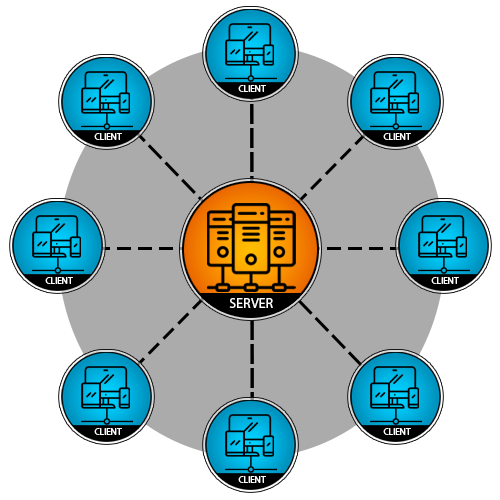
\includegraphics[width=1\linewidth]{content/pictures/ded_server-d5369721966357b9b4d5e1fa96b05b22.png}
\caption{Client-Server-Architektur mit dediziertem Server (Quelle: \cite{noauthor_network_2024})}
\label{fig:dedicated_server}
\end{figure}

\paragraph{Ein Client gehosteter Server} läuft auf demselben Gerät wie die dazugehörige Client-Anwendung (vgl. Abbildung \ref{fig:client_server}).

\begin{figure}[ht]
\centering
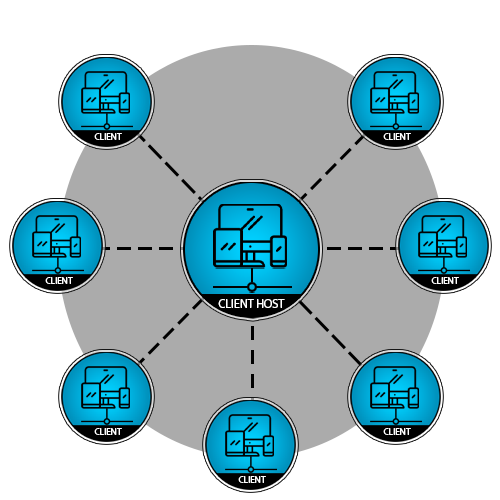
\includegraphics[width=1\linewidth]{content/pictures/client-hosted-16be0b1c9b5020f21325b1e6a7beca73.png}
\caption{Client hosted Server (Quelle: \cite{noauthor_network_2024})}
\label{fig:client_server}
\end{figure}

% \subsection{Client-Side Prediction and Lag Compensation}

% Spiele wie \say{Counterstrike}, \say{Call of Duty}, \say{Valorant} und \say{Apex legends} verwenden ein auf dem klassischen Quake-Modell basierendem Netzwerkmodell. Der Spieler steuert dabei lokal im eigenen Client, auf dem die volle Simulation läuft, ohne dabei Verzögerungen beim Laufen oder Schießen zu haben. Der Server nimmt die Eingaben samt Zeitstempel des Clients entgegen und verteilt den \say{State} zurück. Bspw. das Inventar, Munition oder Feuerraten. Die Korrekturen des \say{State}s werden rückwirkend auf den Client angewandt, der den Zustand bis zur aktuellen Zeit wieder herstellt (\say{Client-Side Prediction}). Schüsse und der damit einhergehende Schaden wir auf dem Server ausgewertet und an die Clients übergeben. Um das Spielerlebnis reaktionsschnell und präzise zu gestatlten, nutzt der Server ein \say{Lag Compensation} Verfahren, bei dem er anhand gespeicherter Zustände die Welt aus der Sicht der Clients zum Schlusspunkt rekonstruiert wird (vgl. \say{}.

\subsection{Peer-to-Peer}
Das \ac{P2P}-Architektur-Modell verbindet jeden Spieler direkt mit allen anderen.Über diese Verbindungen werden Daten zu Spielzuständen und Ereignissen ausgetauscht. Im \say{reinen} \ac{P2P}-System gibt es keinen zentralen \say{Host}. Stattdessen ist jeder Client dafür verantwortlich, seinen eigenen Avatar (oder seine Einheiten) zu verwalten und erhält gleichzeitig Updates von den anderen Clients (vgl. \cite{mygames_unity_2024}). Abbildung \ref{fig:p-2-p} zeigt die entsprechende Topologie.

\begin{figure}[ht]
\centering
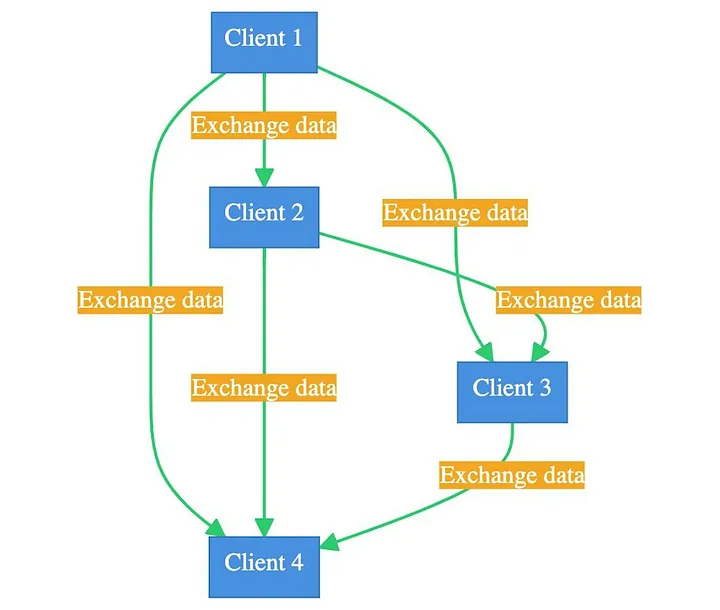
\includegraphics[width=1\linewidth]{content/pictures/0_poGQC2fWQ3tPWPwT.png}
\caption{Peer-to-Peer Infrastruktur (Quelle: \cite{mygames_unity_2024})}
\label{fig:p-2-p}
\end{figure}


\subsection{Relay-Server}
Der Relay-Dienst ermöglicht Multiplayer-Unterstützung ohne die Notwenigkeit eines dedizierten Spielserver. Dabei wird die Kommunikation die Kommunikation zwischen den Spielern über sogenannte Relay-Server weitergeleitet. Nachrichten werden mithilfe einer latenzarmen Datagramm-Übertragung übermittelt, sodass keine direkte Verbindung zwischen den einzelnen Spielern erforderlich ist (vgl. \cite{noauthor_relay_nodate}).

\begin{figure}[ht]
\centering
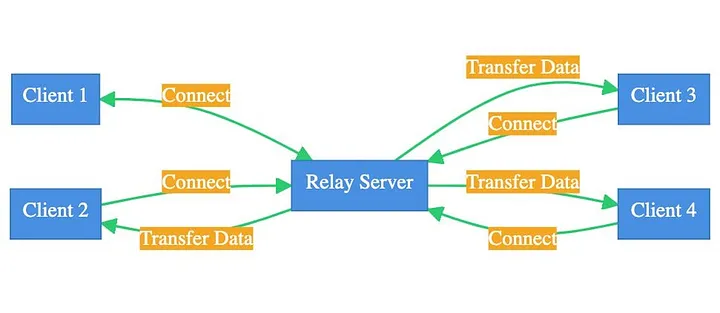
\includegraphics[width=1\linewidth]{content/pictures/0_o7LJU1ImxPHIM5Ej.png}
\caption{Relay-Server Infrastruktur (Quelle: \cite{mygames_unity_2024})}
\label{fig:relay-server}
\end{figure}

% \subsection{Verwendete Kommunikationsprotokolle}
% [überlegung hier noch die protokolle erwähnen]

